\documentclass[border=4pt]{standalone}
\usepackage{tikz}
\usetikzlibrary{positioning, arrows.meta, shapes.geometric, calc, fit, backgrounds}
\usepackage{amsmath,amssymb}
\begin{document}
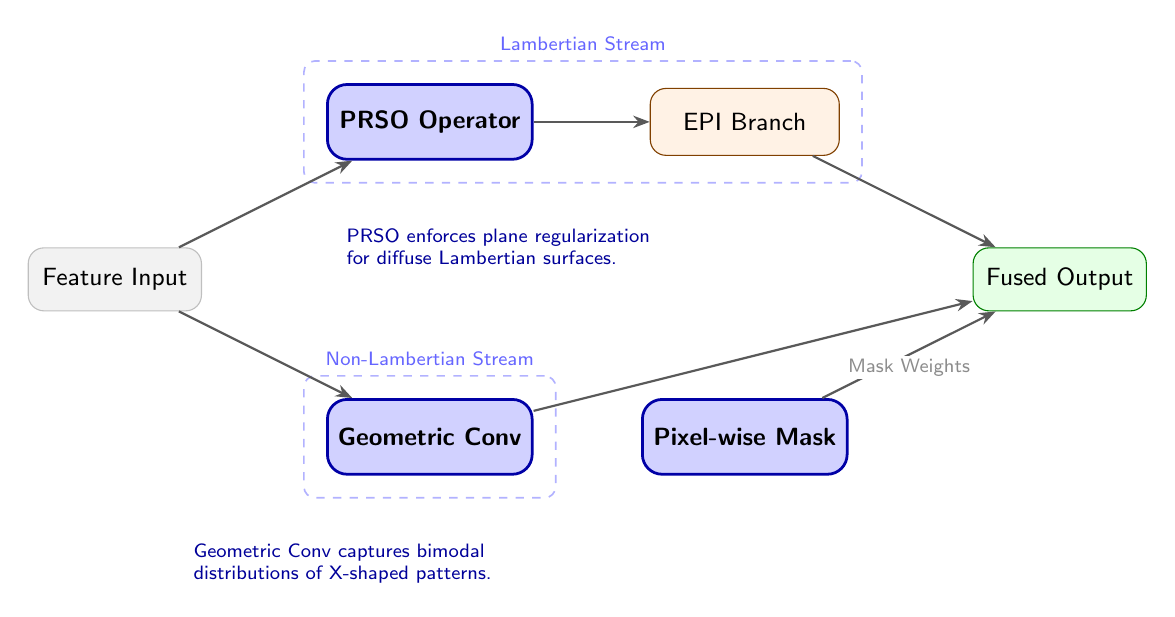
\begin{tikzpicture}[
  node distance=1.5cm and 2.5cm,
  input/.style={draw, rounded corners=2mm, minimum width=2.2cm, minimum height=0.8cm,
                fill=gray!10, draw=gray!50, align=center, font=\sffamily\small},
  innov/.style={draw, rounded corners=2.5mm, minimum width=2.6cm, minimum height=0.95cm,
                fill=blue!18, draw=blue!65!black, line width=1pt, align=center,
                font=\sffamily\small\bfseries},
  proc/.style={draw, rounded corners=2mm, minimum width=2.4cm, minimum height=0.85cm,
               fill=orange!10, draw=orange!50!black, align=center, font=\sffamily\small},
  output/.style={draw, rounded corners=2mm, minimum width=2.2cm, minimum height=0.8cm,
                 fill=green!10, draw=green!50!black, align=center, font=\sffamily\small},
  arr/.style={-{Stealth[length=6pt]}, thick, color=black!65},
  gbox/.style={draw=blue!30, dashed, rounded corners=4pt, inner sep=8pt, line width=0.6pt},
  lbl/.style={font=\sffamily\scriptsize, text=black!45, fill=white, inner sep=1pt},
  note/.style={font=\sffamily\scriptsize, text=blue!60!black, align=left, inner sep=2pt},
]

% Nodes
\node[input] (m1) at (0,0) {Feature Input};
\node[innov] (m2) at (4, 2.0) {PRSO Operator};
\node[proc] (m3) at (8, 2.0) {EPI Branch};
\node[innov] (m4) at (4, -2.0) {Geometric Conv};
\node[innov] (m5) at (8, -2.0) {Pixel-wise Mask};
\node[output] (m6) at (12, 0) {Fused Output};

% Arrows - Main Data Flow
\draw[arr] (m1) -- (m2);
\draw[arr] (m1) -- (m4);
\draw[arr] (m2) -- (m3);
\draw[arr] (m3) -- (m6);
\draw[arr] (m4) -- (m6);
\draw[arr] (m5) -- node[below, lbl, pos=0.5] {Mask Weights} (m6);

% Groups & Annotations
\begin{scope}[on background layer]
  \node[gbox, fit=(m2)(m3), label={[font=\sffamily\scriptsize, text=blue!60]above:Lambertian Stream}] (g1) {};
  \node[gbox, fit=(m4), label={[font=\sffamily\scriptsize, text=blue!60]above:Non-Lambertian Stream}] (g2) {};
\end{scope}

\node[note, below=0.5cm of g1.south, text width=6cm] {PRSO enforces plane regularization\\for diffuse Lambertian surfaces.};
\node[note, below=0.5cm of g2.south, text width=6cm] {Geometric Conv captures bimodal\\distributions of X-shaped patterns.};

\end{tikzpicture}
\end{document}